\chapter{Árvore B}
\label{ch:heap} % This how you label a chapter and the key (e.g., ch:into) will be used to refer this chapter ``Introduction'' later in the report. 

% the key ``ch:into'' can be used with command \ref{ch:intor} to refere this Chapter.
% 
\section*{Introdução}
A Árvore B está inclusa na categoria da árvores autobalanceáveis tal qual as árvores AVL e Rubro-Negra, entretanto o que a diferencia destas são seus nós que podem armazenar mais de um valor chave. Idealizada por Rudolf Bayer e Edward Meyers McCreight, esta tem como fim trabalhar com grandes volumes de dados normalmente armazenados em memória secundária(na época, através de discos rígidos magnéticos). Devido a isso, sua estratégia conceitual consiste em não carregar todos os dados na memória principal, apenas algumas páginas.

Bem como é elucidado na pirâmide de hierarquia de memória, existe uma relação inversamente proporcional entre custo e capacidade de armazenamento de memórias de menor latência.

\begin{figure}[!ht]
	\centering
	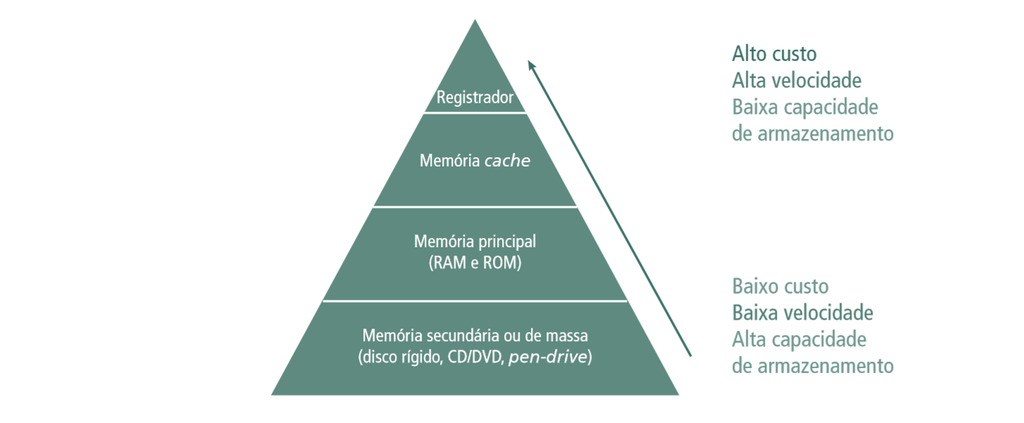
\includegraphics[scale=0.7]{figures/piramide.png}
\end{figure}

Sendo assim, quando se trabalha com um volume significativo de dados é inviável 
\section*{Busca}
Complexidade log n
\section*{Inserção}
Complexidade log n
\section*{Remoção}
Complexidade log n


% \newpage
%
